\documentclass[tikz, margin=5mm]{standalone}

\usepackage{pgfplots}
\pgfplotsset{compat=1.18}

\begin{document}
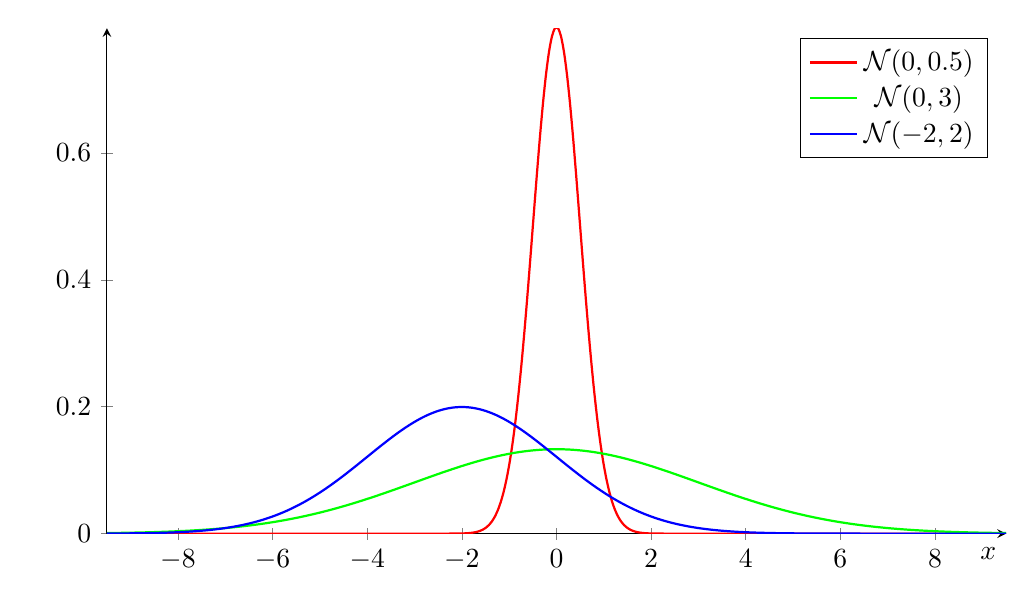
\begin{tikzpicture}
\begin{axis}[
        axis x line=middle,
        axis y line=left,
        domain=-9.5:9.5, smooth, samples=300,
        width=13cm, height=8cm,
        xlabel=$x$, ylabel=\empty,
        xlabel style={yshift=-13pt},
        legend style={at={(0.98,0.98)}, anchor=north east},
]
        \addplot[thick, red] {1/(0.5*sqrt(2*pi))*exp(-((x-0)^2)/(2*0.5^2))};
        \addlegendentry{$\mathcal{N}(0, 0.5)$}
        \addplot[thick, green] {1/(3*sqrt(2*pi))*exp(-((x-0)^2)/(2*3^2))};
        \addlegendentry{$\mathcal{N}(0, 3)$}
        \addplot[thick, blue] {1/(2*sqrt(2*pi))*exp(-((x+2)^2)/(2*2^2))};
        \addlegendentry{$\mathcal{N}(-2, 2)$}
\end{axis}
\end{tikzpicture}
\end{document}